\achapter{18}{The Characteristic Equation} \label{sec:characteristic_equation}

\vspace*{-17 pt}
\framebox{
\parbox{\dimexpr\linewidth-3\fboxsep-3\fboxrule}
{\begin{fqs}
\item What is the characteristic polynomial of a matrix?
\item What is the characteristic equation of a matrix?
\item How and why is the characteristic equation of a matrix useful?
\item How many different eigenvalues can an $n \times n$  matrix have?
\item How large can the dimension of the eigenspace corresponding to an eigenvalue be?
\end{fqs}}}% \hspace*{3 pt}}

\vspace*{13 pt}

\csection{Application: Modeling the Second Law of Thermodynamics}

Pour cream into your cup of coffee and the cream spreads out; straighten up your room and it soon becomes messy again; when gasoline is mixed with air in a car's cylinders, it explodes if a spark is introduced. In each of these cases a transition from a low energy state (your room is straightened up) to a higher energy state (a messy, disorganized room) occurs. This can be described by entropy -- a measure of the energy in a system. Low energy is organized (like ice cubes) and higher energy is not (like water vapor). It is a fundamental property of energy (as described by the second law of thermodynamics) that the entropy of a system cannot decrease. In other words, in the absence of any external intervention, things never become more organized.

The Ehrenfest model\footnote{named after Paul and Tatiana Ehrenfest who introduced it in ``{\"U}ber zwei bekannte Einw{\"a}nde gegen das Boltzmannsche H-Theorem," \emph{Physikalishce Zeitschrift}, vol. 8 (1907), pp. 311-314)} is a Markov process proposed to explain the statistical interpretation of the second law of thermodynamics using the diffusion of gas molecules. This process can be modeled as a problem of balls and bins, as we will do later in this section. The characteristic polynomial of the transition matrix will help us find the eigenvalues and allow us to analyze our model. 


\csection{Introduction}
We have seen that the eigenvalues of an $n \times n$ matrix $A$ are the scalars $\lambda$ so that $A - \lambda I_n$ has a nontrivial null space. Since a matrix has a nontrivial null space if and only if the matrix is not invertible, we can also say that $\lambda$ is an eigenvalue of $A$ if
\begin{equation}
\det(A - \lambda I_n) = 0. \label{eq:PA5.2_1}
\end{equation}
This equation is called the \emph{characteristic equation} of $A$. It provides us an \emph{algebraic} way to find eigenvalues, which can then be used in finding eigenvectors corresponding to each eigenvalue. Suppose we want to find the eigenvalues of $A=\left[ \begin{array}{cc} 1 & 1 \\ 1& 3 \end{array} \right]$. Note that 
\[ A- \lambda I_2 = \left[ \begin{array}{cc} 1-\lambda & 1 \\ 1& 3-\lambda \end{array} \right]\, ,\]
with determinant $(1-\lambda)(3-\lambda)-1=\lambda^2-4\lambda+2$. Hence, the eigenvalues $\lambda_1, \lambda_2$ are the solutions of the characteristic equation $\lambda^2-4\lambda+2=0$. Using quadratic formula, we find that $\lambda_1=2+\sqrt{2}$ and $\lambda_2=2-\sqrt{2}$ are the eigenvalues.

In this activity, our goal will be to use the characteristic equation to obtain information about eigenvalues and eigenvectors of a matrix with real entries.

\begin{pa} \label{pa:4_b} ~

\be
\item For each of the following parts, use the characteristic equation to determine the eigenvalues of $A$. Then, for each eigenvalue $\lambda$, find a basis of the corresponding eigenspace, i.e., $\Nul(A-\lambda I)$. You might want to recall how to find a basis for the null space of a matrix from Section \ref{sec:null_space}. Also, make sure that your eigenvalue candidate $\lambda$ yields nonzero eigenvectors in $\Nul(A-\lambda I)$ for otherwise $\lambda$ will not be an eigenvalue.

	\ba
	\begin{minipage}{1.5in} 
	\item $A=\left[ \begin{array}{cr} 2 &0 \\ 0 & -3 \end{array}\right]$
	\end{minipage}
	\begin{minipage}{1.5in} 
	\item $A=\left[ \begin{array}{cc} 1 & 2 \\ 0 & 1 \end{array}\right]$
	\end{minipage}
	\begin{minipage}{1.5in} 
	\item $A=\left[ \begin{array}{cc} 1 & 4 \\2 & 3 \end{array}\right]$
	\end{minipage}

\ea

\item Use your eigenvalue and eigenvector calculations of the above problem as a guidance to answer the following questions about a matrix with real entries.

\ba
	\item At most how many eigenvalues can a $2\times 2$ matrix have? Is it possible to have no eigenvalues? Is it possible to have only one eigenvalue? Explain.
	
\item If a matrix is an upper-triangular matrix (i.e., all entries below the diagonal are 0's, as in the first two matrices of the previous problem), what can you say about its eigenvalues? Explain.


\item How many linearly independent eigenvectors can be found for a $2\times 2$ matrix? Is it possible to have a matrix without 2 linearly independent eigenvectors? Explain.

\ea

\item Using the characteristic equation, determine which matrices have 0 as an eigenvalue.

\ee

\end{pa}



\csection{The Characteristic Equation}

Until now, we have been given eigenvalues or eigenvectors of a matrix and determined eigenvectors and eigenvalues from the known information. In this section we use determinants to find (or approximate) the eigenvalues of a matrix. From there we can find (or approximate) the corresponding eigenvectors. The tool we will use is a polynomial equation, the \emph{characteristic equation}, of a square matrix whose roots are the eigenvalues of the matrix. The characteristic equation will then provide us with an \emph{algebraic} way of finding the eigenvalues of a square matrix. 

We have seen that the eigenvalues of a square matrix $A$ are the scalars $\lambda$ so that $A - \lambda I$ has a nontrivial null space. Since a matrix has a nontrivial null space if and only if the matrix is not invertible, we can also say that $\lambda$ is an eigenvalue of $A$ if
\begin{equation}
\det(A - \lambda I) = 0. \label{eq:4_b_1}
\end{equation}
Note that if $A$ is an $n \times n$ matrix, then $\det(A - \lambda I)$ is a polynomial of degree $n$. Furthermore, if $A$ has real entries, the polynomial has real coefficients. This polynomial, and the equation (\ref{eq:4_b_1}) are given special names.



\begin{definition} Let $A$ be an $n \times n$ matrix. The \textbf{characteristic polynomial}\index{characteristic polynomial} of $A$ is the polynomial
\[\det(A-\lambda I_n),\]
where $I_n$ is the $n \times n$ identity matrix. The \textbf{characteristic equation}\index{characteristic equation} of $A$ is the equation
\[\det(A-\lambda I_n) = 0.\]
\end{definition}



So the characteristic equation of $A$ gives us an algebraic way of finding the eigenvalues of $A$.



\begin{activity} \label{act:4_b_1} ~
	\ba
	\item Find the characteristic polynomial of the matrix $A = \left[ \begin{array}{crc} 3&-2&5 \\ 1&0&7 \\ 0&0&1 \end{array} \right]$, and use the characteristic polynomial to find all of the eigenvalues of $A$.
	

	
	\item  Verify that 1 and 2 are the only eigenvalues of the matrix $\left[ \begin{array}{cccc} 1&0&0&1\\ 1&2&0&0 \\ 0&0&1&0 \\ 0&0&0&1 \end{array} \right]$.



	\ea
\end{activity}



As we argued in Preview Activity \ref{pa:4_b}, a $2 \times 2$ matrix can have at most 2 eigenvalues. For an $n \times n$ matrix, the characteristic polynomial will be a degree $n$ polynomial, and we know from algebra that a degree $n$ polynomial can have at most $n$ roots. Since an eigenvalue of a matrix is a root of the characteristic polynomial of that matrix, we can conclude that an $n \times n$ matrix can have at most $n$ distinct eigenvalues. Activity \ref{act:4_b_1} (b) shows that a $4 \times 4$ matrix may have fewer than $4$ eigenvalues, however. Note that one of these eigenvalues, the eigenvalue 1, appears three times as a root of the characteristic polynomial of the matrix. The number of times an eigenvalue appears as a root of the characteristic polynomial is called the \emph{(algebraic) multiplicity} of the eigenvalue. More formally:



\begin{definition} The \textbf{(algebraic) multiplicity}\index{multiplicity!algebraic} of an eigenvalue $\lambda$ of a matrix $A$ is the largest integer $m$ so that $(x-\lambda)^m$ divides the characteristic polynomial of $A$.
\end{definition}



Thus, in Activity \ref{act:4_b_1} (b) the eigenvalue 1 has multiplicity 3 and the eigenvalue 2 has multiplicity 1. Notice that if we count the eigenvalues of an $n \times n$ matrix with their multiplicities, the total will always be $n$.

 

If $A$ is a matrix with real entries, then the characteristic polynomial will have real coefficients. It is possible that the characteristic polynomial can have complex roots, and that the matrix $A$ has complex eigenvalues. The Fundamental Theorem of Algebra shows us that if a real matrix has complex eigenvalues, then those eigenvalues will appear in conjugate pairs, i.e., if $\lambda_1=a+ib$ is an eigenvalue of $A$, then $\lambda_2=a-ib$ is another eigenvalue of $A$. Furthermore, for an odd degree polynomial, since the complex eigenvalues will come in conjugate pairs, we will be able to find at least one real eigenvalue.



We now summarize the information we have so far about eigenvalues of an $n\times n$ real matrix:

\begin{theorem} Let $A$ be an $n\times n$ matrix with real entries. Then
\begin{enumerate}
\item There are at most $n$ eigenvalues of $A$. If each eigenvalue (including complex eigenvalues) is counted with its multiplicity, there are exactly $n$ eigenvalues.
\item If $A$ has a complex eigenvalue $\lambda$, the complex conjugate of $\lambda$ is also an eigenvalue of $A$.
%\item There are at most $n$ real eigenvalues of $A$.
\item If $n$ is odd, $A$ has at least one real eigenvalue.
\item If $A$ is upper or lower-triangular, the eigenvalues are the entries on the diagonal.
\end{enumerate}
\end{theorem}



\csection{Eigenspaces, A Geometric Example}

Recall that for each eigenvalue $\lambda$ of an $n \times n$ matrix $A$, the eigenspace of $A$ corresponding to the eigenvalue $\lambda$ is $\Nul (A - \lambda I_n)$. These eigenspaces can tell us important information about the matrix transformation defined by $A$. For example, consider the matrix transformation $T$ from $\R^3$ to $\R^3$ defined by $T(\vx) = A \vx$, where
\[A = \left[ \begin{array}{ccc} 1&0&1\\0&1&1\\0&0&2 \end{array} \right].\]
We are interested in understanding what this matrix transformation does to vectors in $\R^3$. First we note that $A$ has eigenvalues $\lambda_1 = 1$ and $\lambda_2 = 2$, with $\lambda_1$ having multiplicity $2$. There is a pair $\vv_1 = \left[ \begin{array}{c} 1\\0\\0 \end{array} \right]$ and $\vv_2 = \left[ \begin{array}{c} 0\\1\\0 \end{array} \right]$ of linearly independent eigenvectors for $A$ corresponding to the eigenvalue $\lambda_1$ and an eigenvector $\vv_3=\left[ \begin{array}{c} 1\\1\\1 \end{array} \right]$ for $A$ corresponding to the eigenvalue $\lambda_2$. Note that the vectors $\vv_1$, $\vv_2$, and $\vv_3$ are linearly independent (recall from Theorem \label{thm:4_b_lin_indep_evects} that eigenvectors corresponding to different eigenvalues are always linearly independent). So any vector $\vb$ in $\R^3$ can be written uniquely as a linear combination of $\vv_1$, $\vv_2$, and $\vv_3$. Let's now consider the action of the matrix transformation $T$ on a linear combination of $\vv_1$, $\vv_2$, and $\vv_2$. Note that 
\begin{align} 
T(c_1\vv_1 + c_2 \vv_2 + c_3 \vv_3) &= c_1T(\vv_1) + c_2T(\vv_2) + c_3 T(\vv_3) \notag \\
	&= c_1 \lambda_1 \vv_1 + c_2 \lambda_1 \vv_2 + c_3 \lambda_2 \vv_3 \notag \\
	&= (1)(c_1\vv_1 + c_2 \vv_2) + (2)c_3 \vv_3. \label{eq:4_b_2}
\end{align}
Equation (\ref{eq:4_b_2}) illustrates that it is most convenient to view the action of $T$ in the coordinate system where $\Span \{\vv_1\}$ serves as the $x$-axis, $\Span \{\vv_2\}$ serves as the $y$-axis, and $\Span \{\vv_3\}$ as the $z$-axis. In this case, we can visualize that when we apply the transformation $T$ to a vector $\vb = c_1 \vv_1 + c_2 \vv_2 + c_3 \vv_3$ in $\R^3$ the result is an output vector that is unchanged in the $\vv_1$-$\vv_2$ plane and scaled by a factor of $2$ in the $\vv_3$ direction. For example, consider the box whose sides are determined by the vectors $\vv_1$, $\vv_2$, and $\vv_3$ as shown in Figure \ref{F:4_b_1}. The transformation $T$ stretches this box by a factor of $2$ in the $\vv_3$ direction and leaves everything else alone, as illustrated in Figure \ref{F:4_b_1}. So the entire $\Span \{\vv_1, \vv_2\})$ is unchanged by $T$, but $\Span \{\vv_3\})$ is scaled by $2$. In this situation, the eigenvalues and eigenvectors provide the most convenient perspective through which to visualize the action of the transformation $T$. 
\begin{figure}[ht]
\begin{center}
\resizebox{!}{2.3in}{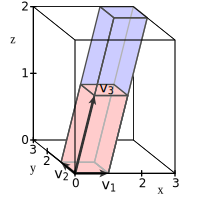
\includegraphics{4_b_Eigenspaces.eps}}
%\resizebox{!}{2.5in}{[trim=1cm 1cm 1cm 1cm, clip]%{4_b_Eigenspaces.png}}
%trim=left bottom right top, clip
\end{center}
\caption{A box and a transformed box.}
\label{F:4_b_1}
\end{figure}

This geometric perspective illustrates how each eigenvalue and the corresponding eigenspace of $A$ tells us something important about $A$. So it behooves us to learn a little more about eigenspaces. 


\csection{Dimensions of Eigenspaces}

There is a connection between the dimension of the eigenspace of a matrix corresponding to an eigenvalue and the multiplicity of that eigenvalue as a root of the characteristic polynomial. Recall that the dimension of a subspace of $\R^n$ is the number of vectors in a basis for the eigenspace. We investigate the connection between dimension and multiplicity in the next activity.



\begin{activity} \label{act:4_b_3} ~
	
	\ba
	\item Find the dimension of the eigenspace for each eigenvalue of matrix $A = \left[ \begin{array}{crc} 3&-2&5 \\ 1&0&7 \\ 0&0&1 \end{array} \right]$ from Activity \ref{act:4_b_1} (a). 
	

	
	\item Find the dimension of the eigenspace for each eigenvalue of matrix $A=\left[ \begin{array}{cccc} 1&0&0&1\\ 1&2&0&0 \\ 0&0&1&0 \\ 0&0&0&1 \end{array} \right]$ from Activity \ref{act:4_b_1} (b).



 \item Consider now a $3\times 3$ matrix with 3 distinct eigenvalues $\lambda_1, \lambda_2, \lambda_3$. 

\begin{enumerate}[i.]
\item Recall that a polynomial of degree can have at most three distinct roots. What does that say about the multiplicities of $\lambda_1, \lambda_2, \lambda_3$?



\item Use the fact that eigenvectors corresponding to distinct eigenvalues are linearly independent to find the dimensions of the eigenspaces for $\lambda_1, \lambda_2, \lambda_3$.

\end{enumerate}



	\ea
\end{activity}



The examples in Activity \ref{act:4_b_3} all provide instances of the principle that the dimension of an eigenspace corresponding to an eigenvalue $\lambda$ cannot exceed the multiplicity of $\lambda$. Specifically:



\begin{theorem} If $\lambda$ is an eigenvalue of $A$, the dimension of the eigenspace corresponding to $\lambda$ is less than or equal to the multiplicity of $\lambda$.
\end{theorem}



The examples we have seen raise another important point. The matrix $A = \left[ \begin{array}{ccc} 1&0&1\\0&1&1\\0&0&2 \end{array} \right]$ from our geometric example has two eigenvalues $1$ and $2$, with the eigenvalue 1 having multiplicity 2. If we let $E_{\lambda}$ represent the eigenspace of $A$ corresponding to the eigenvalue $\lambda$, then $\dim(E_1)=2$ and $\dim(E_2) = 1$. If we change this matrix slightly to the matrix $B = \left[ \begin{array}{crc} 2&0&1 \\ 0&1&1 \\ 0&0&1 \end{array} \right]$ we see that $B$ has two eigenvalues $1$ and $2$, with the eigenvalue 1 having multiplicity 2. However, in this case we have $\dim(E_1) = 1$ (like the example in from Activities \ref{act:4_b_1} (a) and \ref{act:4_b_3} (a)). In this case the vector $\vv_1 = [1 \ 0 \ 0]^{\tr}$ forms a basis for $E_2$ and the vector $\vv_2 = [0 \ 1 \ 0]^{\tr}$ forms a basis for $E_1$. We can visualize the action of $B$ on the square formed by $\vv_1$ and $\vv_2$ in the $xy$-plane as a scaling by 2 in the $\vv_1$ direction as shown in Figure \ref{F:4_b_2}, but since we do not have a third linearly independent eigenvector, the action of $B$ in the direction of $[0 \ 0 \ 1]^{\tr}$ is not so clear. 
\begin{figure}[ht]
\begin{center}
\resizebox{!}{2.3in}{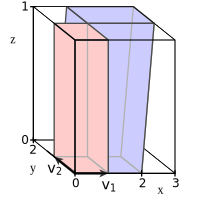
\includegraphics{4_b_Eigenspaces_2.eps}}
%\resizebox{!}{2.5in}{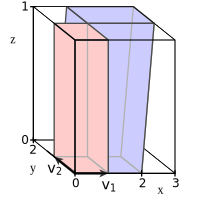
\includegraphics[trim=1cm 1cm 1cm 1cm, clip]{4_b_Eigenspaces_2.png}}
%trim=left bottom right top, clip
\end{center}
\caption{A box and a transformed box.}
\label{F:4_b_2}
\end{figure}

So the action of a matrix transformation can be more easily visualized if the dimension of each eigenspace is equal to the multiplicity of the corresponding eigenvalue. This geometric perspective leads us to define the geometric multiplicity of an eigenvalue.



\begin{definition} The \textbf{geometric multiplicity}\index{multiplicity!geometric} of an eigenvalue of an $n \times n$ matrix $A$ is the dimension of the corresponding eigenspace $\Nul (A-\lambda I_n)$. 
\end{definition}

 
\csection{Examples}

\ExampleIntro

\begin{example} Let $A = \left[ \begin{array}{rcr} -1&0&-2 \\ 2&1&2 \\ 0&0&1 \end{array}\right]$. 
\ba
\item Find the characteristic polynomial of $A$. 

\item Factor the characteristic polynomial and find the eigenvalues of $A$. 

\item Find a basis for each eigenspace of $A$. 

\item Is it possible to find a basis for $\R^3$ consisting of eigenvectors of $A$? Explain. 

\ea


\ExampleSolution
\ba
\item The characteristic polynomial of $A$ is 
\begin{align*}
p(\lambda) &= \det(A - \lambda I_3) \\
	&= \det\left( \left[ \begin{array}{ccc} -1-\lambda&0&-2 \\ 2&1-\lambda&2 \\ 0&0&1-\lambda \end{array}\right] \right) \\
	&= (-1-\lambda)(1-\lambda)(1-\lambda).
\end{align*}

\item The eigenvalues of $A$ are the solutions to the characteristic equation. Since 
\[p(\lambda) = (-1-\lambda)(1-\lambda)(1-\lambda) = 0\]
implies $\lambda = -1$ or $\lambda = 1$, the eigenvalues of $A$ are $1$ and $-1$.

\item To find a basis for the eigenspace of $A$ corresponding to the eigenvalue $1$, we find a basis for $\Nul (A-I_3)$. The reduced row echelon form of $A - I_ 3 = \left[ \begin{array}{rcr} -2&0&-2 \\ 2&0&2 \\ 0&0&0 \end{array}\right]$ is $\left[ \begin{array}{ccc} 1&0&1 \\ 0&0&0 \\ 0&0&0 \end{array}\right]$. If $\vx = \left[ \begin{array}{c} x_1\\x_2\\x_3 \end{array} \right]$, then $(A-I_3)\vx = \vzero$ has general solution 
\[\vx = \left[ \begin{array}{c} x_1\\x_2\\x_3 \end{array} \right] = \left[ \begin{array}{r} -x_3\\x_2\\x_3 \end{array} \right] = x_2 \left[ \begin{array}{c} 0\\1\\0 \end{array} \right] + x_3\left[ \begin{array}{r} -1\\0\\1 \end{array} \right].\]
Therefore, $\{[0 \ 1 \ 0]^{\tr}, [-1 \ 0 \ 1]^{\tr}\}$ is a basis for the eigenspace of $A$ corresponding to the eigenvalue $1$. 

To find a basis for the eigenspace of $A$ corresponding to the eigenvalue $-1$, we find a basis for $\Nul (A+I_3)$. The reduced row echelon form of $A + I_ 3 = \left[ \begin{array}{ccr} 0&0&-2 \\ 2&2&2 \\ 0&0&2 \end{array}\right]$ is $\left[ \begin{array}{ccc} 1&1&0 \\ 0&0&1 \\ 0&0&0 \end{array}\right]$. If $\vx = \left[ \begin{array}{c} x_1\\x_2\\x_3 \end{array} \right]$, then $(A+I_3)\vx = \vzero$ has general solution 
\[\vx = \left[ \begin{array}{c} x_1\\x_2\\x_3 \end{array} \right] = \left[ \begin{array}{r} -x_2\\x_2\\0 \end{array} \right] = x_2 \left[ \begin{array}{r} -1\\1\\0 \end{array} \right].\]
Therefore, a basis for the eigenspace of $A$ corresponding to the eigenvalue $-1$ is $\{[-1 \ 1 \ 0]^{\tr}\}$. 

\item Let $\vv_1 = [0 \ 1 \ 0]^{\tr}, [-1 \ 0 \ 1]^{\tr}$, $\vv_2 =  [-1 \ 0 \ 1]^{\tr}$, and $\vv_3 =  [-1 \ 1 \ 0]^{\tr}$. Since eigenvectors corresponding to different eigenvalues are linearly independent, and since neither $\vv_1$ nor $\vv_2$ is a scalar multiple of the other, we can conclude that the set $\{\vv_1, \vv_2, \vv_3\}$ is a linearly independent set with $3 = \dim(\R^3)$ vectors.  Therefore, $\{\vv_1, \vv_2, \vv_3\}$ is a basis for $\R^3$ consisting of eigenvectors of $A$. 

\ea

\end{example}

\begin{example} Find a $3 \times 3$ matrix $A$ that has an eigenvector $\vv_1 = [1 \ 0 \ 1]^{\tr}$ with corresponding eigenvalue $\lambda_1 = 2$, an eigenvector $\vv_2 = [0 \ 2 \ -3]^{\tr}$ with corresponding eigenvalue $\lambda_2 = -3$, and an eigenvector $\vv_3 = [-4 \ 0 \ 5]^{\tr}$ with corresponding eigenvalue $\lambda_3 = 5$. Explain your process. 

\ExampleSolution
We are looking for a $3 \times 3$ matrix $A$ such that $A \vv_1 = 2 \vv_1$, $A \vv_2 = -3 \vv_2$ and $A \vv_3 = 5 \vv_3$. Since $\vv_1$, $\vv_2$, and $\vv_3$ are eigenvectors corresponding to different eigenvalues, $\vv_1$, $\vv_2$, and $\vv_3$ are linearly independent. So the matrix $[\vv_1 \ \vv_2 \ \vv_3]$ is invertible. It follows that 
\begin{align*}
A[\vv_1 \ \vv_2 \ \vv_3] &= [A\vv_1 \ A\vv_2 \ A\vv_3] \\
A \left[\begin{array}{rcr} 1&0&-4 \\ 0&2&0 \\ 1&-3&5 \end{array} \right] &= [2\vv_1 \ -3\vv_2 \ 5\vv_3] \\
A \left[\begin{array}{crr} 1&0&-4 \\ 0&2&0 \\ 1&-3&5 \end{array} \right] &= \left[ \begin{array}{crr} 2&0&-20 \\ 0&-6&0 \\ 2&9&25 \end{array} \right] \\
A &=  \left[ \begin{array}{crr} 2&0&-20 \\ 0&-6&0 \\ 2&9&25 \end{array} \right] \left[\begin{array}{crr} 1&0&-4 \\ 0&2&0 \\ 1&-3&5 \end{array} \right]^{-1}\\
A &= \left[ \begin{array}{crr} 2&0&-20 \\ 0&-6&0 \\ 2&9&25 \end{array} \right]  \left[\renewcommand{\arraystretch}{1.4} \begin{array}{rcc} \frac{5}{9}&\frac{2}{3}&\frac{4}{9} \\ 0&\frac{1}{2}&0 \\ -\frac{1}{9}&\frac{1}{6}&\frac{1}{9} \end{array} \right]\\
A &= \left[\renewcommand{\arraystretch}{1.4} \begin{array}{rrr} \frac{10}{3}&-2&-\frac{4}{3} \\ 0&-3&0 \\ -\frac{5}{3}&10&\frac{11}{3} \end{array} \right].
\end{align*}



\end{example}

\csection{Summary}
In this section we studied the characteristic polynomial of a matrix and similar matrices.
\begin{itemize}
\item If $A$ is an $n \times n$ matrix, the characteristic polynomial of $A$ is the polynomial
\[\det(A-\lambda I_n),\]
where $I_n$ is the $n \times n$ identity matrix.
\item If $A$ is an $n \times n$ matrix, the characteristic equation of $A$ is the equation
\[\det(A-\lambda I_n) = 0.\]
\item The characteristic equation of a square matrix provides us an algebraic method to find the eigenvalues of the matrix.
\item The eigenvalues of an upper or lower-triangular matrix are the entries on the diagonal.
\item There are at most $n$ eigenvalues of an $n\times n$ matrix.
\item For a real matrix $A$, if an eigenvalue $\lambda$ of $A$ is complex, then the complex conjugate of $\lambda$ is also an eigenvalue.
\item The algebraic multiplicity of an eigenvalue $\lambda$ is the multiplicity of $\lambda$ as a root of the characteristic equation.
\item The dimension of the eigenspace corresponding to an eigenvalue $\lambda$ is less than or equal to the algebraic multiplicity of $\lambda$.

\end{itemize}





\csection{Exercises}
\be
	
\item \label{ex:determinant_eigenvalues} There is a useful relationship between the determinant and eigenvalues of a matrix $A$ that we explore in this exercise. 
	\ba
	\item Let $B = \left[ \begin{array}{cc} 2&3\\8&4 \end{array} \right]$. Find the determinant of $B$ and the eigenvalues of $B$, and compare $\det(B)$ to the eigenvalues of $B$.
	
	\item Let $A$ be an $n \times n$ matrix. In this part of the exercise we argue the general case illustrated in the previous part -- that $\det(A)$ is the product of the eigenvalues of $A$. Let $p(\lambda) = \det(A - \lambda I_n)$ be the characteristic polynomial of $A$.
		\begin{enumerate}[i.]
		\item Let $\lambda_1$, $\lambda_2$, $\ldots$, $\lambda_n$ be the eigenvalues of $A$ (note that these eigenvalues may not all be distinct). Recall that if $r$ is a root of a polynomial $q(x)$, then $(x-r)$ is a factor of $q(x)$. Use this idea to explain why 
	\[p(\lambda) = (-1)^{n} (\lambda-\lambda_1)(\lambda- \lambda_2) \cdots (\lambda - \lambda_n).\]
		\item Explain why $p(0) = \lambda_1 \lambda_2 \cdots \lambda_n$. 
		\item Why is $p(0)$ also equal to $\det(A)$. Explain how we have shown that $\det(A)$ is the product of the eigenvalues of $A$. 
		\end{enumerate}
	\ea


	
\item Find the eigenvalues of the following matrices. For each eigenvalue, determine its algebraic and geometric multiplicity.

\ba
\item $A=\left[ \begin{array}{ccc} 1&1&1\\1&1&1\\1&1&1\end{array} \right]$

\item $A=\left[ \begin{array}{ccc} 2&0&3\\0&1&0\\0&1&2\end{array} \right]$
\ea

\item Let $A$ be an $n \times n$ matrix. Use the characteristic equation to explain why $A$ and $A^\tr$ have the same eigenvalues.

\item Find three $3 \times 3$ matrices whose eigenvalues are 2 and 3, and for which the dimensions of the eigenspaces for $\lambda=2$ and $\lambda=3$ are different. 

\item Suppose $A$ is an $n\times n$ matrix and $B$ is an invertible $n\times n$ matrix. Explain why the characteristic polynomial of $A$ is the same as the characteristic polynomial of $BAB^{-1}$, and hence, as a result, the eigenvalues of $A$ and $BAB^{-1}$ are the same.

\item Label each of the following statements as True or False. Provide justification for your response.
\ba

\item \textbf{True/False} If the determinant of a $2 \times 2$ matrix $A$ is positive, then $A$ has two distinct real eigenvalues.

\item \textbf{True/False} If two $2 \times 2$ matrices have the same eigenvalues, then the have the same eigenvectors. 

\item \textbf{True/False} The characteristic polynomial of an $n \times n$ matrix has degree $n$.

\item \textbf{True/False} If $R$ is the reduced row echelon form of an $n \times n$ matrix $A$, then $A$ and $R$ have the same eigenvalues. 

\item \textbf{True/False} If $R$ is the reduced row echelon form of an $n \times n$ matrix $A$, and $\vv$ is an eigenvector of $A$, then $\vv$ is an eigenvector of $R$. 

\item \textbf{True/False} Let $A$ and $B$ be $n \times n$ matrices with characteristic polynomials $p_A(\lambda)$ and $p_B(\lambda)$, respectively. If $A \neq B$, then $p_A(\lambda) \neq p_B(\lambda)$. 

\item \textbf{True/False}  Every matrix has at least one eigenvalue. 

\item \textbf{True/False}  Suppose $A$ is a $3 \times 3$ matrix with three distinct eigenvalues. Then any three eigenvectors, one for each eigenvalue, will form a basis of $\R^3$.

\item \textbf{True/False} If an eigenvalue $\lambda$ is repeated 3 times among the eigenvalues of a matrix, then there are at most 3 linearly independent eigenvectors corresponding to $\lambda$.


\ea

\ee

\csection{Project: The Ehrenfest Model}

To realistically model the diffusion of gas molecules we would need to consider a system with a large number of balls as substitutes for the gas molecules. However, the main idea can be seen in a model with a much smaller number of balls, as we will do now. Suppose we have two bins that contain a total of $4$ balls between them. Label the bins as Bin 1 and Bin 2. In this case we can think of entropy as the number of different possible ways the balls can be arranged in the system. For example, there is only $1$ way for all of the balls to be in Bin 1 (low entropy), but there are $4$ ways that we can have one ball in Bin 1 (choose any one of the four different balls, which can be distinguished from each other) and $3$ balls in Bin 2 (higher entropy). The highest entropy state has the balls equally distributed between the bins (with $6$ different ways to do this).

We assume that there is a way for balls to move from one bin to the other (like having gas molecules pass through a permeable membrane). A way to think about this is that we select a ball (from ball 1 to ball 4, which are different balls) and move that ball from its current bin to the other bin. Consider a ``move" to be any instance when a ball changes bins. A \emph{state} is any configuration of balls in the bins at a given time, and the state changes when a ball is chosen at random and moved to the other bin. The possible states are to have 0 balls in Bin 1 and 4 balls in Bin 2 (State 0, entropy 1), 1 ball in Bin 1 and 3 in Bin 2 (State 1, entropy 4), 2 balls in each Bin (State 2, entropy 6), 3 balls in Bin 1 and 1 ball in Bin 2 (State 3, entropy 4), and 4 balls in Bin 1 and 0 balls in Bin 2 (State 4, entropy 1). These states are shown in Figure \ref{F:Ehrenfest}.

\begin{figure}[h]
\begin{center}
\resizebox{!}{2.5in}{
\includegraphics{4_b_states}}
\end{center}
\caption{States}
\label{F:Ehrenfest}
\end{figure}

%\begin{figure}[h]
%\begin{center}
%\begin{minipage}{1in}
%\begin{center}
%\resizebox{!}{1.0in}{\includegraphics{x0}}
%\end{center}
%\end{minipage}
%\begin{minipage}{1in}
%\begin{center}
%\resizebox{!}{1.0in}{\includegraphics{x1}}
%\end{center}
%\end{minipage}
%\begin{minipage}{1in}
%\begin{center}
%\resizebox{!}{1.0in}{\includegraphics{x2}}
%\end{center}
%\end{minipage} %\\
%\begin{minipage}{1in}
%\begin{center}
%\resizebox{!}{1.0in}{\includegraphics{x3}}
%\end{center}
%\end{minipage}
%\begin{minipage}{1in}
%\begin{center}
%\resizebox{!}{1.0in}{\includegraphics{x4}}
%\end{center}
%\end{minipage}
%\end{center}
%\caption{States}
%\label{F:Ehrenfest}
%\end{figure}


\begin{pactivity} \label{act:Eherenfest_model} To model the system of balls in bins we need to understand how the system can transform from one state to another. It suffices to count the number of balls in Bin 1 (since the remaining balls will be in Bin 2). Even though the balls are labeled, our count only cares about how many balls are in each bin. Let $\vx_0 = [x_0, x_1, x_2, x_3, x_4]^{\tr}$, where $x_i$ is the probability that Bin 1 contains $i$ balls, and let $\vx_1 = \left[ x_0^1, x_1^1, x_2^1, x_3^1, x_4^1 \right]^{\tr}$, where $x_i^1$ is the probability that Bin 1 contains $i$ balls after the first move. We will call the vectors $\vx_0$ and $\vx_1$ \emph{probability distributions} of balls in bins. Note that since all four balls have to be placed in some bin, the sum of the entries in our probability distribution vectors must be $1$. Recall that a move is an instance when a ball changes bins. We want to understand how $\vx_1$ is obtained from $\vx_0$. In other words, we want to figure out what the probability that Bin 1 contains 0, 1, 2, 3, or 4 balls after one ball changes bins if our initial probability distribution of balls in bins is $\vx_0$. 

We begin by analyzing the ways that a state can change. For example, 
\begin{itemize}
\item Suppose there are $0$ balls in Bin 1. (In our probability distribution $\vx_0$, this happens with probability $x_0$.) Then there are four balls in Bin 2. The only way for a ball to change bins is if one of the four balls moves from Bin 2 to Bin 1, putting us in State 1. Regardless of which ball moves, we will always be put in State 1, so this happens with a probability of $1$. In other words, if the probability that Bin 1 contains $0$ balls is $x_0$, then there is a probability of $(1)x_0$ that Bin 1 will contain 1 ball after the move. 

\item Suppose we have 1 ball in Bin 1. There are four ways this can happen (since there are four balls, and the one in Bin 1 is selected at random from the four balls), so the probability of a given ball being in Bin 1 is $\frac{1}{4}$. 
	\begin{itemize}
	\item If the ball in Bin 1 moves, that move puts us in State $0$. In other words, if the probability that Bin 1 contains 1 ball is $x_1$, then there is a probability of $\frac{1}{4}x_1$ that Bin 1 will contain $0$ balls after a move.
	\item If any of the $3$ balls in Bin 2 moves (each moves with probability $\frac{3}{4}$), that move puts us in State 2. In other words, if the probability that Bin 1 contains 1 ball is $x_1$, then there is a probability of $\frac{3}{4}x_1$ that Bin 1 will contain $2$ balls after a move.
	\end{itemize}
\end{itemize}

\ba
\item Complete this analysis to explain the probabilities if there are $2$, $3$, or $4$ balls in Bin 1.

\item Explain how the results of part (a) show that 
\begin{center}
\setlength{\tabcolsep}{.26667em}
\begin{tabular}{rcccccccccc} \\
$x_0^1$ &= &$0x_0$ &+ &$\frac{1}{4} x_1$	&+  &$0 x_2$ 				&+ &$0 x_3$ 				&+ &$0 x_4$ \\
$x_1^1$ &= &$1x_0$ &+ &$0 x_1$ 			    &+ &$\frac{1}{2} x_2$	    &+  &$0 x_3$ 				&+  &$0 x_4$ \\
$x_2^1$ &= &$0x_0$ &+ &$\frac{3}{4} x_1$ 	&+ &$0 x_2$ 				&+ &$\frac{3}{4} x_3$ 	    &+ &$0 x_4$ \\
$x_3^1$ &= &$0x_0$ &+ &$0 x_1$ 			    &+ &$\frac{1}{2} x_2$ 	    &+ &$0 x_3$ 				&+ &$1 x_4$ \\
$x_4^1$ &= &$0x_0$ &+ &$0 x_1$ 			    &+ &$0 x_2$ 				&+ &$\frac{1}{4} x_3$	    &+ &$0 x_4$ \\
\end{tabular}
\end{center}

\ea

\end{pactivity}

The system we developed in Project Activity \ref{act:Eherenfest_model} has matrix form
\[\vx_1 = T \vx_0,\]
where $T$ is the \emph{transition matrix}
\[T = \left[ \renewcommand{\arraystretch}{1.2} \begin{array}{ccccc}
0 & \frac{1}{4}	& 0 			& 0 			& 0 \\
1 & 0 			& \frac{1}{2}	& 0 			& 0 \\
0 & \frac{3}{4} & 0 			& \frac{3}{4} 	& 0 \\
0 & 0 			& \frac{1}{2} 	& 0 			& 1 \\
0 & 0 			& 0 			& \frac{1}{4}	& 0 \\
\end{array} \right].\]

Subsequent moves give probability distribution vectors 
\begin{align*}
\vx_2 &= T\vx_1 \\
\vx_3 &= T\vx_2  \\
\vdots & \hspace{0.2in} \vdots \\
\vx_k &= T\vx_{k-1} .
\end{align*}

This example is an example of a Markov process (see Definition \ref{def:Markov}). There are several questions we can ask about this model. For example, what is the long-term behavior of this system, and how does this model relate to entropy? That is, given an initial probability distribution vector $\vx_0$, the system will have probability distribution vectors $\vx_1$, $\vx_2$, $\ldots$ after subsequent moves. What happens to the vectors $\vx_k$ as $k$ goes to infinity, and what does this tell us about entropy? To answer these questions, we will first explore the sequence $\{\vx_k\}$ numerically, and then use the eigenvalues and eigenvectors of $T$ to analyze the sequence $\{\vx_k\}$. 

\begin{pactivity} \label{act:Ehrenfest_numeric} Use appropriate technology to do the following.
	\ba
	\item Suppose we begin with a probability distribution vector $\vx_0 = [1 \ 0 \ 0 \ 0 \ 0]^{\tr}$. Calculate vectors $\vx_k$ for enough values of $k$ so that you can identify the long term behavior of the sequence. Describe this behavior.
	
	\item Repeat part (a) with 
	\begin{enumerate}[i.]
	\item $\vx_0 = \left[0 \ \frac{1}{2} \ \frac{1}{2} \ 0 \ 0\right]^{\tr}$
	\item $\vx_0 = \left[0 \ \frac{1}{3} \ \frac{1}{3} \ 0 \ \frac{1}{3}\right]^{\tr}$
	\item $\vx_0 = \left[\frac{1}{5} \ \frac{1}{5} \ \frac{1}{5} \ \frac{1}{5} \ \frac{1}{5}\right]^{\tr}$
	\end{enumerate}
	Describe the long term behavior of the sequence $\{\vx_k\}$ in each case. 
	

	\ea
	
\end{pactivity}

In what follows, we investigate the behavior of the sequence $\{\vx_k\}$ that we uncovered in Project Activity \ref{act:Ehrenfest_numeric}.

\begin{pactivity} \label{act:Ehrenfest_eigenvalues} We use the characteristic polynomial to find the eigenvalues of $T$.  
    \ba
    \item Find the characteristic polynomial of $T$. Factor the characteristic polynomial into a product of linear polynomials to show that the eigenvalues of $T$ are $0$, $1$, $-1$, $\frac{1}{2}$ and $-\frac{1}{2}$. 
    

	\item As we will see a bit later, certain eigenvectors for $T$ will describe the end behavior of the sequence $\{\vx_k\}$. Find eigenvectors for $T$ corresponding to the eigenvalues $1$ and $-1$. Explain how the eigenvector for $T$ corresponding to the eigenvalue $1$ explains the behavior of one of the sequences was saw in Project Activity \ref{act:Ehrenfest_numeric}. (Any eigenvector of $T$ with eigenvalue $1$ is called an \emph{equilibrium} or \emph{steady state} vector.) 


\ea
\end{pactivity}

Now we can analyze the behavior of the sequence $\{\vx_k\}$.

\begin{pactivity} \label{act:Ehrenfest_basis} To make the notation easier, we will let $\vv_1$ be an eigenvector of $T$ corresponding to the eigenvalue $0$, $\vv_2$ an eigenvector of $T$ corresponding to the eigenvalue $1$, $\vv_3$ an eigenvector of $T$ corresponding to the eigenvalue $-1$, $\vv_4$ an eigenvector of $T$ corresponding to the eigenvalue $\frac{1}{2}$, and $\vv_5$ an eigenvector of $T$ corresponding to the eigenvalue $-\frac{1}{2}$. 

	\ba
	
	\item Explain why $\{\vv_1, \vv_2, \vv_3, \vv_4, \vv_5\}$ is a basis of $\R^5$.
    
	\item Let $\vx_0$ be any initial probability distribution vector. Explain why we can write $\vx_0$ as
\[\vx_0 = a_1 \vv_1 + a_2 \vv_2 + a_3 \vv_3 + a_4 \vv_4 + a_5 \vv_5 = \sum_{i=1}^5 a_i \vv_i\]
for some scalars $a_1$, $a_2$, $a_3$, $a_4$, and $a_5$.

\ea

\end{pactivity}


We can now use the eigenvalues and eigenvectors of $T$ to write the vectors $\vx_k$ in a convenient form. Let $\lambda_1 = 0$, $\lambda_2=1$, $\lambda_3=-1$, $\lambda_4=\frac{1}{2}$, and $\lambda_5=-\frac{1}{2}$. Notice that 
\begin{align*}
\vx_1 &= T \vx_0  \\
	&= T(a_1  \vv_1 + a_2 \vv_2 + a_3  \vv_3 + a_4  \vv_4 + a_5 \vv_5) \\
	&= a_1  T\vv_1 + a_2 T\vv_2 + a_3  T\vv_3 + a_4 T\vv_4 + a_5 T\vv_5 \\
	&= a_1\lambda_1 \vv_1 + a_2\lambda_2 \vv_2 + a_3 \lambda_3 \vv_3 + a_4 \lambda_4 \vv_4 + a_5 \lambda_5 \vv_5 \\
	&= \sum_{i=1}^5 a_i \lambda_i \vv_i.
\end{align*}
Similarly
\[\vx_2 = T \vx_1 = T\left(\sum_{i=1}^5 a_i \lambda_i\vv_i\right) = \sum_{i=1}^5 a_i \lambda_i T\vv_i = \sum_{i=1}^5 a_i\lambda_i^2 \vv_i.\]
We can continue in this manner to ultimately show that for each positive integer $k$ we have 
\begin{equation} \label{eq:Ehrenfest_sum}
\vx_k = \sum_{i=1}^5 a_i\lambda_i^k \vv_i
\end{equation}
when $\vx_0 = \sum_{i=1}^5 a_i \vv_i$. 


\begin{pactivity} \label{act:Ehrenfest_entropy} Recall that we are interested in understanding the behavior of the sequence $\{\vx_k\}$ as $k$ goes to infinity.
	\ba
	\item Equation (\ref{eq:Ehrenfest_sum}) shows that we need to know $\lim_{k \to \infty} \lambda_i^k$ for each $i$ in order to analyze $\lim_{k \to \infty} \vx_k$. Calculate or describe these limits.    

	\item Use the result of part (a), Equation (\ref{eq:Ehrenfest_sum}), and Project Activity \ref{act:Ehrenfest_eigenvalues} (b) to explain why the sequence $\{\vx_k\}$ is either eventually fixed or oscillates between two states. Compare to the results from Project Activity \ref{act:Ehrenfest_numeric}. How are these results related to entropy? You may use the facts that 
\begin{itemize}
\item $\vv_1 = [1 \ 0 \ -2 \ 0 \ 1]^{\tr}$ is an eigenvector for $T$ corresponding to the eigenvalue $0$,
\item $\vv_2 = [1 \ 4 \ 6 \ 4 \ 1]^{\tr}$ is an eigenvector for $T$ corresponding to the eigenvalue $1$,
\item $\vv_3 = [1 \ -4 \ 6 \ -4 \ 1]^{\tr}$ is an eigenvector for $T$ corresponding to the eigenvalue $-1$,
\item $\vv_4 = [-1 \ -2 \ 0\ 2 \ 1]^{\tr}$ is an eigenvector for $T$ corresponding to the eigenvalue $\frac{1}{2}$,
\item $\vv_5 = [-1 \ 2 \ 0 \ -2 \ 1]^{\tr}$ is an eigenvector for $T$ corresponding to the eigenvalue $-\frac{1}{2}$.
\end{itemize}

	
\ea

\end{pactivity}


